\chapter{Background}

In this chapter, we shall discuss various research areas with particular focus on established and experimental APIs and transport protocols. Each research area's connection to this project's aims shall be outlined and gaps in current research will be highlighted as motivation for this project.

\section{WebRTC}
% https://csperkins.org/publications/2021/01/rfc8834.txt RTP with WebRTC
% https://dl.acm.org/doi/pdf/10.1145/3199524.3199534 performance eval of webrtc-based video conferencing

WebRTC is an open-source protocol suite that aims to allow developers to easily implement cross-platform, real-time communication of video, audio or generic data via a range of APIs in their applications. Initially released in 2011, the project has since been widely adopted and is supported by many organisations including Apple, Google, Microsoft and Mozilla \cite{webrtc.org}. The World Wide Web Consortium (W3C) manages a JavaScript API that allows developers to implement WebRTC into their applications whilst the Internet Engineering Task Force (IETF) handles the underlying protocols and security mechanisms. Since its release, WebRTC's adoption has been widespread - the majority of modern devices that utilise video or voice data can natively use the protocols or utilise technologies based on them \cite{gross_2020}.

A WebRTC peer may be a user endpoint (peer-to-peer implementation) or may act as a server between user endpoints (client-server implementation). WebRTC sends media data (audio and video) via the SRTP (Secure Real-time Transport Protocol) protocol; SRTP data packets are carried within UDP. Additionally, WebRTC provides a peer-to-peer or client-server, bidirectional data channel that utilises SCTP (Stream Control Transmission Protocol) in a secure UDP tunnel. The data channel supports congestion control, re-transmissions, multiple sub-streams, message-oriented abstraction, framed messages, and can be configured to adjust reliable and ordered properties \cite{webrtc-sctp}. 

\begin{figure}[h]
    \centering
    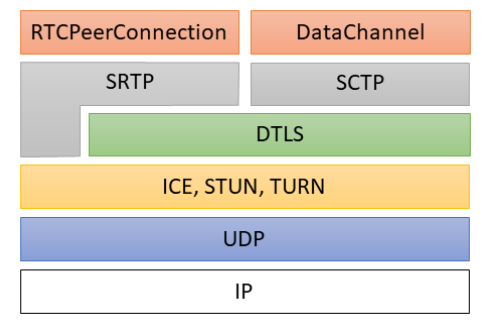
\includegraphics[width=0.4\columnwidth]{images/WebRTC connection stack.png}
	\caption{WebRTC Stack Diagram \cite{garcia2020}}
    \label{webrtc_connection_stack}
\end{figure}

\subsection{SCTP}

A core issue with WebRTC is the use of SCTP in its data channel. SCTP was originally designed for use as a signalling protocol and therefore was intended to transfer small amounts of data. This becomes problematic in scenarios where an application is required to send large amounts of data can result in critical data being blocked. \cite{webrtc_mozilla} This is relevant as although WebRTC could potentially migrate to using QUIC rather than SCTP, with new APIs designed with QUIC in mind emerging (i.e. WebTransport), it may be phased out. 

\subsection{Connection Establishment}

To establish peer-to-peer connections, WebRTC utilises the ICE algorithm which in turn makes use of the STUN and TURN protocols. Here, WebRTC attempts to make a connection directly utilising the peer address - if this fails, the ICE algorithm obtains an external address via a STUN server provided by the peer and if this fails, the algorithm finally routes traffic via a TURN relay server provided by the peer. \cite{jadhav2021} According to the documentation of Google's open-source library named "libjingle", 8\% of WebRTC connections require the use of TURN servers and therefore the end-to-end delay of a WebRTC connection is often increased due to media relay. \cite{garcia2019} This is relevant to us as QUIC achieves 0-RTT (round trip time) connection establishment - this implies that WebTransport (which uses QUIC) would have faster connection establishment than WebRTC. We know this because the ICE algorithm that WebRTC utilises is not designed with timeliness in mind. ICE will probe all of a host's candidate IP addresses and ports; although these are assigned priorities based on how likely the host thinks it is to reach a destination address, it can and often does still take a considerable amount of time. QUIC, however, is designed with timeliness as one of its main philosophies - it does not need to waste time probing as it knows exactly what it is connecting to.

\subsection{Handling packet loss with forward error correction}

In the event of packet loss, re-transmission of packets often takes too long in real-time networked applications to be useful - this is particularly prevalent in video conferencing applications where frames of video need to be played out as soon as possible. Instead, SRTP (the transport protocol utilised by WebRTC) utilises forward error correction (FEC) to combat packet loss. This works by sending additional FEC packets that contain error correcting codes alongside the original data. Then, if original packets are lost and FEC packets still arrive, the original data can be reconstructed in a timely manner. 

\subsection{Developer Experience}

Another core issue with WebRTC is that although its high-level API makes development very simple, it means that the algorithm details are hidden from developers and therefore the flexibility of WebRTC is very limited. This becomes an issue in scenarios such as the one presented in a 2013 study on WebRTC and mobile video-conferencing - this study found that WebRTC had "a heavy reliance on packet loss (among other factors) as an indicator of congestion" and that this lead to "underutilization of the wireless channel and poor video quality" \cite{fund2013}. This issue would be negated if developers had access to WebRTC's congestion control algorithm. This is relevant as WebTransport was designed to grant the developer much more flexibility by "[abstracting] away the specific underlying protocol with a flexibile (sic) set of possible capabilities" \cite{wtexplainer}.

However, other aspects of development are made significantly easier due to the widespread support of the API. Notably, further APIs have been developed to simplify various aspects of the WebRTC API - for example, PeerJS is a library that provides a configurable API built on top of WebRTC that greatly simplifies the connection establishment process from a developer's perspective. This kind of community support is not available for WebTransport as it is a far younger API - however, this may change in the future.

A key conclusion noted in several studies is that WebRTC performance degrades considerably in unstable network conditions \cite{moulay2018} \cite{jansen2018} \cite{fund2013}. This is relevant as, once again, having the capability to tailor our video conferencing applications to situations where network conditions may be unstable could be one of WebTransport's strengths.

All web-based conferencing tools today use WebRTC in some capacity \cite{gross_2020}. Popular applications such as Discord, Zoom's web client, Cisco WebEx and Microsoft Teams all utilise WebRTC in various capacities \cite{discord} \cite{webrtc_mozilla_blog}.

\section{QUIC}

QUIC is an emerging transport protocol that aims to replace TCP, TLS and parts of HTTP by acting as a secure, flexible and fast way of transporting data. QUIC supports reliable and ordered data transfer through the use of streams, and also supports unreliable, disordered data transfer by utilising datagrams. QUIC runs over UDP, but incorporates TCP's best practices, notably congestion control and time-based loss detection \cite{iyengar} (both useful features for video conferencing applications). First announced in 2012, QUIC has since been standardised in 2021.

\subsection{Streams and Datagrams}

QUIC has two main methods for transmitting data: by utilising streams \cite{rfc9000} or datagrams \cite{quic-datagrams-draft}. 

Streams provide reliable and ordered transmission of data; this is currently the main non-experimental way to transmit data within QUIC. QUIC is capable of maintaining and utilising multiple streams within a single connection - this is known as "stream multiplexing" and is a significant advantage of QUIC over TCP as it can result in more efficient data transfer. QUIC packets are sent within UDP datagrams along these streams. It is important to note that order is not preserved between these streams; for example, if a message was sent on "Stream A" before a message was sent on "Stream B", there is no guarantee that the message on "Stream A" will arrive before "Stream B"'s. However, QUIC does have the capability to prioritise particular streams and explicitly specify how queued data is transferred across multiple streams. Another important factor of QUIC streams to consider is that message boundaries are not preserved between packets. This can be disadvantageous for developers as it means that additional parsing of packets is required if developers, for example, rely on specific headers to implement application functionality. 
Streams are not ideal for real-time video transfer for numerous reasons. Particularly, their reliable nature results in re-transmission of media data when it already "has passed its play-out deadline and is no longer needed" \cite{perkins2018}. 

Datagrams provide unreliable, disordered and timely transmission of data. Currently, QUIC's implementation of datagrams is considered experimental. The draft proposing this extension states that datagrams would be useful in applications that transmit real-time data as it would combine the unreliable data transfer of UDP and the secure nature of QUIC streams. \cite{quic-datagrams-draft} 
Palmer \textit{et al.} suggest that QUIC be extended to support unreliable streams - their study proposes that there is a "clear use case for a selectively or partially reliable transport, where an application can seamlessly multiplex reliable and unreliable streams over a single connection". \cite{palmer2018} It is important to note that unreliable streams are technically different to datagrams, but the aims and overall achievements of both are the same. In a video streaming scenario, the study suggests that important frames of media data could be sent along reliable streams where as unimportant frames could be sent along unreliable streams. Palmer \textit{et al.} submitted these suggestions as a draft to the QUIC Working Group. \cite{palmerdraft}
Perkins and Ott \cite{perkins2018} advise that this proposal was flawed as it would need "relatively sophisticated APIs to offer fine-grained control of the (re-)transmission and scheduling". This is relevant as WebTransport satisfies this requirement.

\subsection{UDP Deployment}

QUIC runs over UDP for two reasons: to reduce risk of ossification due to middleboxes \cite{ossification} and to ease end-system deployment in user-space apps \cite{quic-udp-deployment}. Ossification is where developers of protocols such as QUIC reach a point where they cannot alter the protocols significantly because doing so would interact poorly with middleboxes that have come to rely on the preexisting nature of such protocols. Middleboxes are deployed by network operators to monitor and modify traffic - common examples include NATs and firewalls. Ossification is less likely to occur because QUIC is designed to make it difficult or impossible for middleboxes to interfere with QUIC connections - it does this by encrypting as much data as possible and ensuring that middleboxes therefore cannot rely on any of a QUIC packet's fields, hence preventing ossification. Additionally, UDP packets are more likely to get through firewalls than TCP packets, thus further preventing ossification. This is relevant as if we are looking for a new technology such as WebTransport to succeed WebRTC, we need to ensure that it will have significant longevity and avoid ossification. Moreover, QUIC being built on UDP further strengthens WebTransport's case for being this successor as having an easy deployment into existing or new applications is key for the potential widespread adoption of WebTransport.  

\begin{figure}[h]
    \centering
    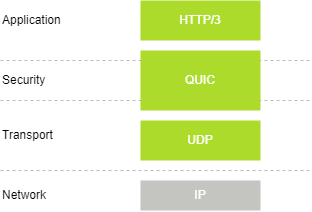
\includegraphics[width=0.5\columnwidth]{images/quic.png}
	\caption{QUIC Stack Diagram}
    \label{webrtc_connection_stack}
\end{figure}


\subsection{Connection Establishment}

A key feature of QUIC is its fast connection establishment. QUIC has a speed improvement over TLS as it combines the connection establishment and TLS handshake into 1 RTT \cite{rfc9000}. QUIC also supports 0-RTT session reestablishment \cite{quic-0rtt}. 
% \todo{Make sure this is true - work on details} 
This is relevant as one of the main conclusions of the aforementioned 2013 study on WebRTC and mobile video-conferencing was that the researchers desired a method to adapt the video data delivery depending on wireless channel conditions using all available information \cite{fund2013}.  A WebTransport implementation could utilise QUIC's 0-RTT connection reestablishment to adapt video data transmission by, for example, switching to sending data via datagrams instead of streams during periods of network instability and quickly reestablishing the session if required. This argument is further strengthened by a 2018 study that found that QUIC was able to start media streams quicker than TCP (WebRTC is likely to use TCP during connection establishment), particularly when there is congestion in the network \cite{arisu2018}. 

\section{WebTransport}

WebTransport is an API that supports streams, datagrams and communication with a remote server via a secure, multiplexed transport. WebTransport runs on top of HTTP/3, which in turn utilises QUIC extensively for data transport and connection establishment \cite{vvv-webtransport-http3-03}. WebTransport was added to Chrome 97 (stable build) in January 2022 \cite{chrome97}. The API is interacted with via JavaScript.

\subsection{Goals}

WebTransport has three goals \cite{wtexplainer}. Firstly, the API aims to provide a low latency method of communication with servers. Secondly, the API aims to be flexible; WebTransport is designed to be utilised for many use cases and with many different network protocols and data transmission configurations. This particular point is what sets it apart from WebRTC, which is less adaptable. Finally, WebTransport aims to achieve the same security properties as its contemporaries, citing WebSockets as a goal - WebSockets uses TLS and server-controlled origin policy. 
% \todo{elaborate on websockets stuff}

\subsection{Use Cases}

As mentioned before, WebTransport aims to be flexible enough to have many use cases. However, one mentioned use case from the Explainer document \cite{wtexplainer} is particularly interesting in a video conferencing scenario - this is "Receiving media pushed from server with minimal latency (out-of-order)". 

\subsection{Streams}
WebTransport is capable of utilising unidirectional and bidirectional streams via HTTP/3 in order to facilitate ordered and reliable data transfer. These streams can be initiated by either endpoint in a client/server connection. The transport of data is then facilitated via QUIC streams. \cite{vvv-webtransport-http3-03}.

\subsection{Datagrams}
WebTransport is capable of sending datagrams by utilising HTTP/3 Datagrams in order to facilitate disordered, unreliable and timely data transfer. \cite{vvv-webtransport-http3-03}. HTTP/3 sends these datagrams by employing the previously discussed experimental QUIC Datagram extension \cite{quic-datagrams-draft}. 
One potential drawback of datagrams stated by the Explainer document is that they are more suited for "small, out-of-order, unreliable messages" with "less API complexity and less network overhead than streams" \cite{wtexplainer}. Video data is quite large and may generate considerable network overhead, so it is therefore worth evaluating transmitting this data via datagrams and streams.



% can we talk about QuicTransport here?
% still not entirely sure on the relationship between the two
% say it has been added to Chrome in January
% other potential uses e.g. games

% \section{HTTP/3} 
% % do I need this?

% \section{Transferring Video Data}


% What did other people do, and how is it relevant to what you want to do?
% \section{Guidance}
% \begin{itemize}    
%     \item
%       Don't give a laundry list of references.
%     \item
%       Tie everything you say to your problem.
%     \item
%       Present an argument.
%     \item Think critically; weigh up the contribution of the background and put it in context.    
%     \item
%       \textbf{Don't write a tutorial}; provide background and cite
%       references for further information.
% \end{itemize}

%==================================================================================================================================